\subsection{Scrum Revisited}
We will revisit Scrum one final time, and discuss the Scrum Retrospective and Scrum Review.
\subsubsection{Scrum Review}
At this point, the final sprint has come to an end, and we review what we have done in this sprint. We will review the backlog and evaluate how well they cover our use cases, so a team potentially could develop more on the program in the future.  \\
\newline
% Move to beginning of Sprint 3
\begin{figure}[H]
  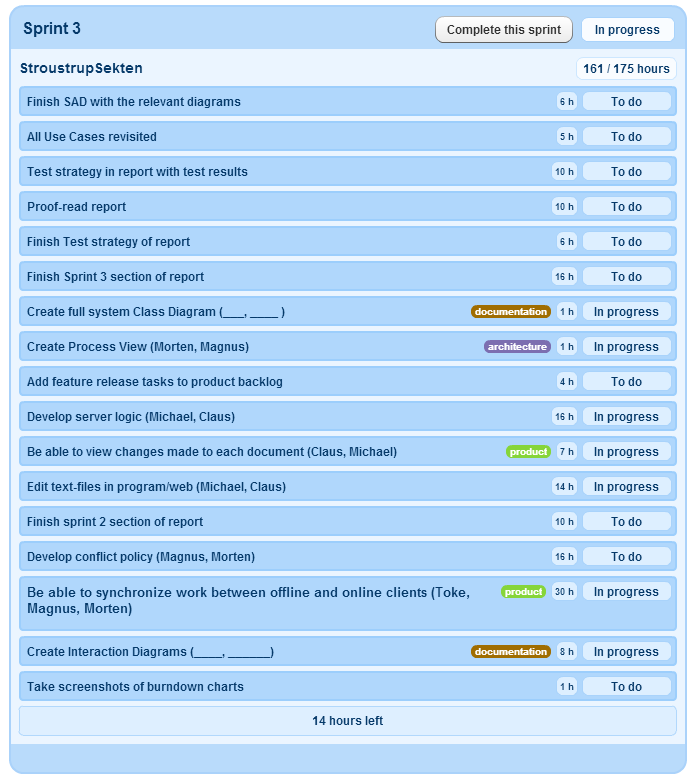
\includegraphics[width=\textwidth]{illustrations/sprint3backlog.PNG}
  \caption{Sprint 3 Backlog}
  \label{sprint3backlog}
\end{figure}
\textbf{Meeting summary}\\
The planned stories for the sprint was finished within the time limits. Most importantly, the hand-in deadline was met.\\
The program is a functioning proof of concept, but one should look at it as a initiated development process, that needs further development to be a program of industrial quality. We have made several aspects of our program open for extensions:
\begin{itemize}
\item Document is an extension of the super-class file. This opens up for extending the program to support other file-types.
\item We have implemented synchronization between several users.
\item We can synchronize several files at the same time, which is much more flexible, than having to synchronize every time a file is saved.
\end{itemize}
These extensions are not fully implemented, but further development in these areas has been made easy and accessible.
In this sprint, we have added functionality to the GUI's such as Changes and Sharing of documents. To measure how well our solution lives up to the requirements, we measure it against the use cases. We have support of:
\begin{itemize}
\item Use Case 1 - Create document offline
\item Use Case 2 - Synchronize changes
\item Use Case 3 - Multiple user edit 
\item Use Case 4 - View version history
\item Use Case 5 - Create document online
\item Use Case 6 - Edit document online
\end{itemize}
\subsubsection{Scrum Retrospective}
We cover this in the conclusion.\\
\newline
The Retrospective and Review concludes our description and discussion of the Scrum we have applied. Additional images of our applied Scrum is available in the Appendix [Appendix, Illustrations, Scrum, page \pageref{scrumillustrations}]
\newpage